% fig5_two_opt — 2-opt flip & affected segments (增量电量校验, 创新点3)
% 用途: 交底书 图5, §五 S3: 翻转子段只重算受影响边 O(k) + 子段内部电池可行性
% 对应: heuristic.py _try_2opt_move (a3_python/heuristic.py:478-557)
% 编译: latexmk -pdf -xelatex fig5_two_opt.tex
\documentclass[tikz,border=8pt]{standalone}
\usepackage{tikz}
\usetikzlibrary{arrows.meta}
\begin{document}
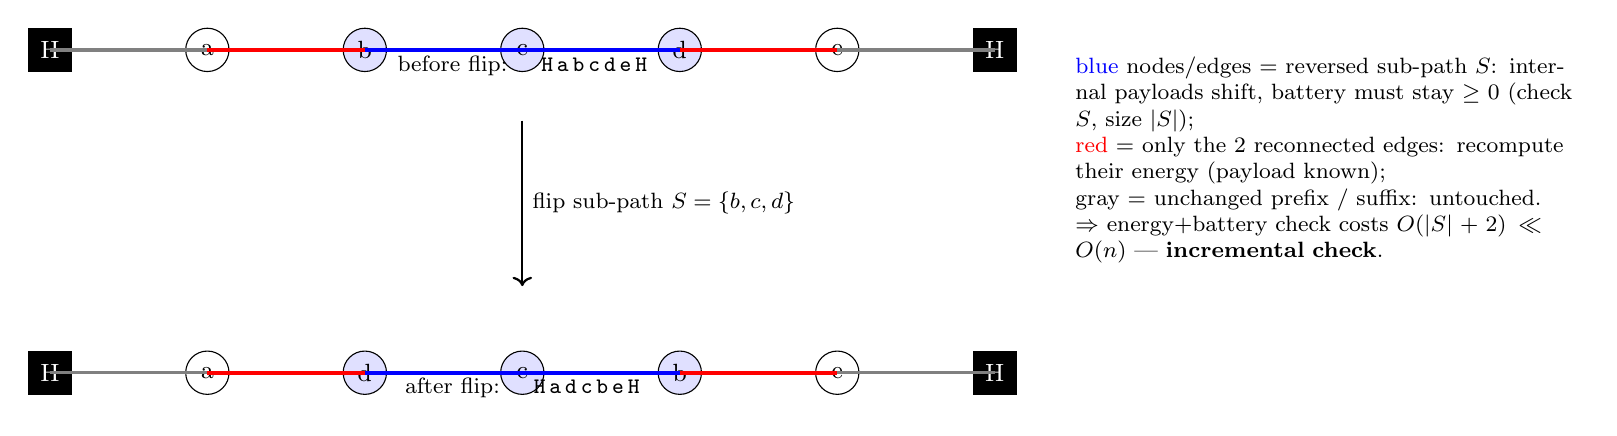
\begin{tikzpicture}[font=\small,
  pt/.style={circle,draw,fill=white,inner sep=0pt,minimum size=0.55cm},
  hpt/.style={rectangle,draw,fill=black,text=white,inner sep=0pt,minimum size=0.55cm},
  nf/.style={fill=blue!12},
]
% ---------------- BEFORE (top) ----------------
\coordinate (A1) at (0,0);
\coordinate (a1) at (2,0);
\coordinate (b1) at (4,0);
\coordinate (c1) at (6,0);
\coordinate (d1) at (8,0);
\coordinate (e1) at (10,0);
\coordinate (A2) at (12,0);
\node[hpt] at (A1) {H}; \node[pt] at (a1) {a};
\node[pt,nf] at (b1) {b}; \node[pt,nf] at (c1) {c}; \node[pt,nf] at (d1) {d};
\node[pt] at (e1) {e};  \node[hpt] at (A2) {H};
\draw[gray,line width=1.2pt] (A1)--(a1);
\draw[red, line width=1.5pt] (a1)--(b1);
\draw[blue,line width=1.5pt] (b1)--(c1) (c1)--(d1);
\draw[red, line width=1.5pt] (d1)--(e1);
\draw[gray,line width=1.2pt] (e1)--(A2);
\node[anchor=north,font=\footnotesize] at (6,0.05) {before flip: \quad \texttt{H\,a\,b\,c\,d\,e\,H}};

% ---------------- AFTER (bottom) ----------------
\coordinate (B1) at (0,-4.1);
\coordinate (a2) at (2,-4.1);
\coordinate (d2) at (4,-4.1);
\coordinate (c2) at (6,-4.1);
\coordinate (b2) at (8,-4.1);
\coordinate (e2) at (10,-4.1);
\coordinate (B2) at (12,-4.1);
\node[hpt] at (B1) {H}; \node[pt] at (a2) {a};
\node[pt,nf] at (d2) {d}; \node[pt,nf] at (c2) {c}; \node[pt,nf] at (b2) {b};
\node[pt] at (e2) {e};  \node[hpt] at (B2) {H};
\draw[gray,line width=1.2pt] (B1)--(a2);
\draw[red, line width=1.5pt] (a2)--(d2);
\draw[blue,line width=1.5pt] (d2)--(c2) (c2)--(b2);
\draw[red, line width=1.5pt] (b2)--(e2);
\draw[gray,line width=1.2pt] (e2)--(B2);
\node[anchor=north,font=\footnotesize] at (6,-4.05) {after flip: \quad \texttt{H\,a\,d\,c\,b\,e\,H}};

% ---------------- annotations ----------------
\draw[->, thick] (6,-0.9) -- (6,-3.0) node[midway,right,font=\footnotesize] {flip sub-path $S=\{b,c,d\}$};
\node[anchor=west,align=left,text width=6.4cm,font=\footnotesize] at (12.9,-1.4)
  {\textcolor{blue}{blue} nodes/edges = reversed sub-path $S$: internal payloads shift, battery must stay $\ge 0$ (check $S$, size $|S|$);\\
   \textcolor{red}{red} = only the 2 reconnected edges: recompute their energy (payload known);\\
   gray = unchanged prefix / suffix: untouched.\\
   $\Rightarrow$ energy+battery check costs $O(|S|+2)\ll O(n)$ --- \textbf{incremental check}.};
\end{tikzpicture}
\end{document}
